% Begin the document and set up the style of the document
\documentclass[a4paper]{article}

% Install the required packages for the document 
\usepackage{envmath}
\usepackage{esvect}
\usepackage{graphicx}
\usepackage{gensymb}
\usepackage{tikz}
\usepackage{geometry}
\usepackage{enumitem}
\usepackage{mathtools}
\usepackage{graphicx}
\usepackage{amsmath}
\usepackage{amscd}
\usepackage{amssymb}
\usepackage{amsfonts}
\usepackage{pgf}
\usepackage{tikz}
\usepackage{mathrsfs}
\usepackage{asyalign}
\usepackage{physics}
\usepackage{cite}
\usepackage{url}
\usepackage[tableposition=top]{caption}
\usepackage{ifthen}
\usepackage[utf8]{inputenc}
\usetikzlibrary{arrows}

\begin{document}

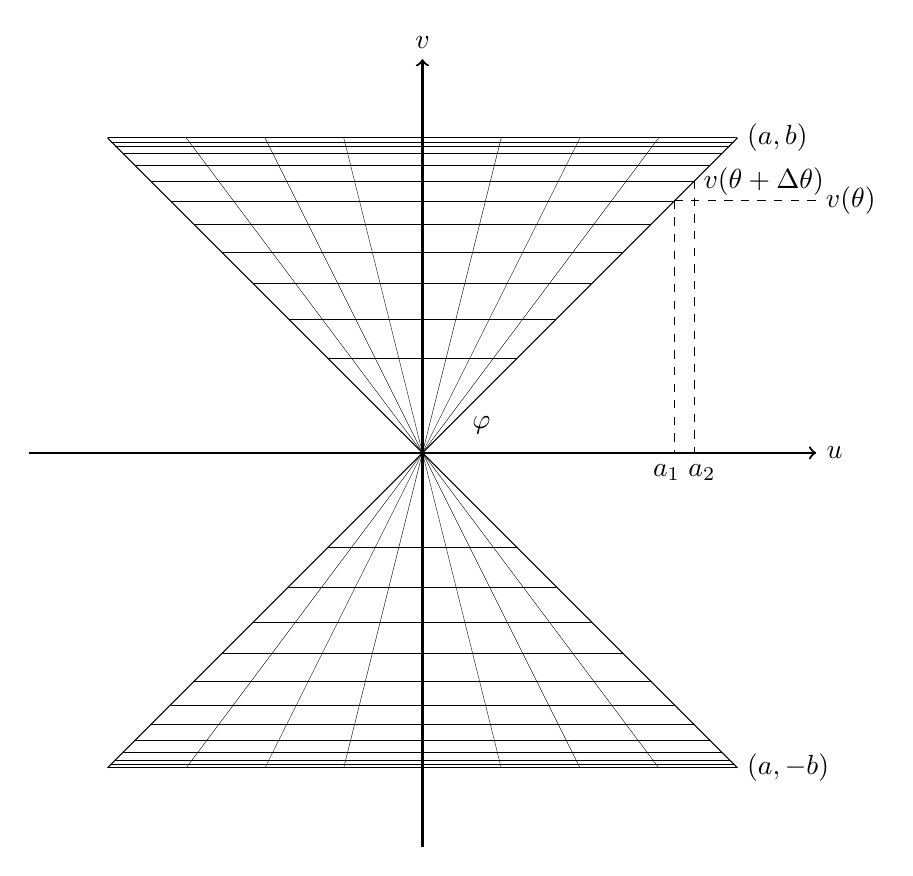
\begin{tikzpicture}
	% X - axis
	\draw[->,thick] (-5,0)--(5,0) node[right]{$u$};
	% Y - axis
	\draw[->,thick] (0,-5)--(0,5) node[above]{$v$};
	% Lines for the meridians 
	\draw (-4,-4 ) -- (4,4);
	\draw [line width=0.05mm] (-3,-4 ) -- (3,4);
	\draw [line width=0.05mm] (-2,-4 ) -- (2,4);
	\draw [line width=0.05mm] (-1,-4 ) -- (1,4);
	\draw [line width=0.05mm] (0,-4 ) -- (0,4);
	\draw [line width=0.05mm] (1,-4 ) -- (-1,4);
	\draw [line width=0.05mm] (2,-4 ) -- (-2,4);
	\draw [line width=0.05mm] (3,-4 ) -- (-3,4);
	\draw (4,-4 ) -- (-4,4);
	\draw (-4,4 ) -- (4,4) node[right]{$(a,b)$};
	\draw (-4,-4 ) -- (4,-4) node[right]{$(a,-b)$};

	\draw [line width=0.05mm] (-3.95,3.95) -- (3.95,3.95);
	\draw [line width=0.05mm] (-3.9,3.9) -- (3.9,3.9);
	\draw [line width=0.05mm] (-3.8,3.8) -- (3.8,3.8);
	\draw [line width=0.05mm] (-3.65,3.65) -- (3.65,3.65);
	\draw [line width=0.05mm] (-3.45,3.45) -- (3.45,3.45) node[right]{$v(\theta + \Delta \theta)$};
	\draw [line width=0.05mm] (-3.2,3.2) -- (3.2,3.2);
	\draw [line width=0.05mm] (-2.9,2.9) -- (2.9,2.9);
	\draw [line width=0.05mm] (-2.55,2.55) -- (2.55,2.55);
	\draw [line width=0.05mm] (-2.15,2.15) -- (2.15,2.15);
	\draw [line width=0.05mm] (-1.7,1.7) -- (1.7,1.7);
	\draw [line width=0.05mm] (-1.2,1.2) -- (1.2,1.2);

	\draw[dashed] (3.45,3.45) -- (3.45,0);
	\node at (3.55,-0.25) {$a_2$};
	\draw[dashed] (3.2,3.2) -- (3.2,0);
	\node at (3.10,-0.25) {$a_1$};
	\draw[dashed] (3.2,3.2) -- (5,3.2) node[right]{$v(\theta)$};

	\draw [line width=0.05mm] (-3.95,-3.95) -- (3.95,-3.95);
	\draw [line width=0.05mm] (-3.9,-3.9) -- (3.9,-3.9);
	\draw [line width=0.05mm] (-3.8,-3.8) -- (3.8,-3.8);
	\draw [line width=0.05mm] (-3.65,-3.65) -- (3.65,-3.65);
	\draw [line width=0.05mm] (-3.45,-3.45) -- (3.45,-3.45);
	\draw [line width=0.05mm] (-3.2,-3.2) -- (3.2,-3.2);
	\draw [line width=0.05mm] (-2.9,-2.9) -- (2.9,-2.9);
	\draw [line width=0.05mm] (-2.55,-2.55) -- (2.55,-2.55);
	\draw [line width=0.05mm] (-2.15,-2.15) -- (2.15,-2.15);
	\draw [line width=0.05mm] (-1.7,-1.7) -- (1.7,-1.7);
	\draw [line width=0.05mm] (-1.2,-1.2) -- (1.2,-1.2);

	\node at (0.75,0.35) {$\varphi$};

\end{tikzpicture}










\end{document}